\documentclass[a4paper, ]{article}
\usepackage[left=2cm, right=2cm, bottom=2.5cm, top=2.5cm]{geometry}

\usepackage[utf8]{inputenc}
\usepackage{amsmath}
\usepackage{amsfonts}
\usepackage{amssymb}
\usepackage{commath}
\usepackage{lipsum}
\usepackage{adjustbox}
\usepackage{float}
\usepackage{hyperref}
\usepackage{graphicx}
\usepackage{gensymb}
\usepackage[spanish]{babel}

\usepackage{multicol}
\usepackage{listings}
\usepackage{enumitem}
\usepackage{booktabs}

\usepackage{multicol}
\title{\Huge{\vspace{-1em}La(s) hoja(s) de Chema}}
\author{}
\date{}
\makeatletter



\usepackage[dvipsnames]{xcolor}

\usepackage{wrapfig}

\usepackage{fancyhdr}
\pagestyle{fancy}
\lhead{Alex Martínez Ascensión}
\chead{}
\rhead{\today}


\usepackage{fourier}

\usepackage[T1]{fontenc}
%\usepackage[default]{gillius}
\usepackage{Alegreya}


\setlength{\parskip}{1em}
\setlength{\parindent}{0em}

\usepackage[
type={CC},
modifier={by-nc-nd},
version={3.0},
]{doclicense}

\setlength{\parindent}{0em}
\setlength{\parskip}{1.1em}
\renewcommand{\baselinestretch}{1.15}
\setlength\itemsep{0em}


\newenvironment{itemizex}%
{\begin{itemize}[noitemsep]%
		\setlength{\itemsep}{0 em}%
		\setlength{\parskip}{0pt}
				\vspace*{-1em}
	}%
	{\end{itemize}}



\newcommand{\dd}{\ensuremath{\operatorname{d}}}
\renewcommand{\d}[1]{\ensuremath{\operatorname{d}\!{#1}}}
\newcommand{\R}{\mathbb{R}}
\renewcommand{\P}{\mathbb{P}}
\newcommand{\m}{\text{medio}}
\newcommand{\iso}{\text{Isom}}
\newcommand{\sen}{\text{sen}}
\usepackage{calrsfs}
\DeclareMathAlphabet{\pazocal}{OMS}{zplm}{m}{n}

\definecolor{azul}{HTML}{107896}
\definecolor{naranja}{HTML}{C2571A}
\definecolor{rojo}{HTML}{9A2617}
\definecolor{amarillo}{HTML}{BCA136}
\definecolor{verde}{HTML}{829356}
\definecolor{gris}{HTML}{909090}
\definecolor{rosa}{HTML}{F9A7B0}
\definecolor{amarillochillon}{HTML}{FBB117}

\newcommand{\axioma}[1]{\textcolor{naranja}{\textbf{Axioma #1}}}
\newcommand{\tma}[1]{\textcolor{rojo}{\textbf{Teorema #1}}}
\newcommand{\defi}[1]{\textcolor{azul}{\textbf{Definición #1}}}
\newcommand{\obs}[1]{\textcolor{verde}{\textbf{Observación #1}}}
\newcommand{\ejem}[1]{\textcolor{verde}{\textbf{Ejemplo #1}}}
\newcommand{\ej}[1]{\textcolor{amarillo}{\textbf{Ejercicio #1}}}
\newcommand{\lema}[1]{\textcolor{rosa}{\textbf{Lema #1}}}
\newcommand{\cor}[1]{\textcolor{rosa}{\textbf{Corolario #1}}}

\newcommand{\dem}[1]{\textcolor{gris}{\normalsize{Demostración. #1}}}

\newcommand{\importante}{\textcolor{amarillochillon}{\textbf{\danger} \,}}



\begin{document}
		\maketitle

	\fontsize{12pt}{12pt}\selectfont
	\vspace*{-4em}
	
	\begin{multicols}{2}
	[
	\section{Espacios métricos}
	]
	
	\defi{1.1} $\delta: M \times M \rightarrow \R $ es una métrica o \textbf{distancia} si cumple que 
	\begin{itemizex}
		\item $\delta(x,y) > 0$ si $x \neq y$, o $\delta(x,x) = 0$
		\item $\delta(x,y) = \delta(y,x)$
		\item $\delta(x,z) \le \delta(x,y) + \delta(y,z)$
	\end{itemizex}
	
	\ej{1.1} Por inducción, la desigualdad triangular se puede generalizar a: $\delta(p^1, p^n) \le \delta(p^1, p^2) + \cdots + \delta(p^{n-1}, p^n)$
	
	\tma{1.4} Si $M' \subset M$ y existe el espacio métrico $(M, \delta)$, entonces también existe $(M', \delta)$, y se llama \textbf{métrica inducida} por $(M,\delta)$.
	
	\defi{1.5} Sean $(M,\delta), (M', \delta')$ y $g: M \rightarrow M'$. Se dice que $g$ conserva las distancias si $\delta'(g(x), g(y)) = \delta(x, y)\;\; \forall \; \; x,y \in M$. Si además $g$ es biyectiva, entonces es una \textbf{isometría}.
	
	\tma{1.7} Si existen $(M, \delta), (M', \delta'), (M'', \delta'')$ y $g: M\rightarrow M'$ y $h: M\rightarrow M'$ son isometrías, entonces $h\circ g$ y $g^{-1}$ también son isometrías.
	
	\defi{1.8} La composición de isometrías forma un \textbf{grupo} pues
	\begin{itemizex}
		\item $(g \circ h) \circ i = g \circ (h \circ i)$
		\item Si $g \in \text{Isom}(M)$ entonces $g^{-1} \in \text{Isom}(M)$
		\item La isometría identidad, $\text{id}_M \in \text{Isom}(M)$
	\end{itemizex}
	
	\defi{1.12} Si $(M, \delta)$, para $a,b \in M$ se llama \textbf{segmento} de extremos $a$ y $b$ y se representa por $[a,b]$ al conjunto $[a,b] = \{x \in M \;|\; \delta(a,x) + \delta(x,b) = \delta(a,b) \}$. Asimismo, $x,y,z \in M$ están alineados si ($x < y < z$) $y \in [x,z]$.	 
	
	\ej{1.5} Para $\sigma \in \{1,-1\}$ y $\tau \in \R$, la aplicación $f(x) = \sigma x+\tau$ es una isometría para $(\R, d_{\R})$
	

	 
	 
	 
	 
	 
	 
	 
	\end{multicols}
	
	\pagebreak
	\textcolor{gris}{\textit{Page intentionally left in blank}}
	\newpage
	\pagebreak
	
	
	\begin{multicols*}{2}
	[\section{Axiomas para la geometría euclidiana plana}]
		\axioma{P1} Si tenemos el conjunto $\P$, denominado \textbf{plano}, y la aplicación $d:\P \times \P \rightarrow \R$ llamada \textbf{distancia}, entonces$(\P, d)$ es un espacio métrico.

\defi{2.2} Una \textbf{recta} $r \subset \P$ satisface
\begin{itemizex}
	\item $r$ contiene al menos dos puntos.
	\item Para toda terna de puntos $A, B, C$, están alineados si están en $r$.
\end{itemizex}

\axioma{P2} $\P$ contiene al menos tres puntos no alineados; y por dos puntos distintos, $A$ y $B$ de $\P$ pasa una recta, $r_{AB}$.

\defi{2.6} / \tma{2.7} Dos rectas se cortan si sólo tienen un punto en común, y si no tienen ningún punto en común, entonces se denominan \textbf{paralelas}, y se denota por $a \parallel b$. Dos rectas, o se cortan o son paralelas.

\importante\axioma{P3} Para toda recta $r \subset \P$ existe una biyección $\gamma: r \rightarrow \R$ tal que $|\gamma(X) - \gamma(Y)| = |x - y| = d(X, Y) \;\; \forall \;\; X,Y \in r$ 

\obs{2.8} Si $A, B \in r$ son distintos, entonces existe un punto $M\in r: d(A,M) = d(M,B)$ que denotamos por $\m[A,B]$ y se llama \textbf{punto medio}. Asimismo sólo existe un punto $B \in r$ tal que $B = \m[A, M]$.

\obs{2.9} Si $r$ es una recta y $P \in r$, entonces $r$ se puede dividir en dos \textbf{semirrectas}, que son los conjuntos $\{X \in r \; | \; \gamma(X) > \gamma(P)\}$ y $\{X \in r \; | \; \gamma(X) < \gamma(P)\}$.

\axioma{P4} Para toda recta $r \subset \P$ hay dos subconjuntos $H^1$ y $H^2$, denominados \textbf{semiplanos} de $r$, que verifican:
\begin{itemizex}
	\item $H^1 \cup H^2 = \P-r$
	\item Si $X,Y \in H^i$ entonces $[X,Y] \subset H^i$
	\item Si $X \in H^1$ y $Y \in H^2$ entonces $[X,Y] \cap r \neq \emptyset$.
\end{itemizex}

\defi{2.15} Sean $P, Q, R$ no alineados, entonces el triángulo $\triangle\{P,Q,R\}$, o $\triangle PQR$ está formado por los segmentos $[P,Q]$, $[Q,R]$, $[P,R]$, llamados lados, y los vértices $P,Q, R$.

\tma{2.16 [Axioma de Pasch]a} Dado un triángulo $\triangle PQR$ y una recta $r$; si $r$ corta a $[P,Q]$, entonces o corta a $[P,R]$ o a $[Q, R]$.

\defi{2.17 = 1.5} Una \textbf{isometría} en $\P$ es una biyección $g: \P \rightarrow \P$ que cumple que $d(g(X), g(Y)) = d(X,Y) \;\;\forall\;\; X,Y \in \P$.

\tma{2.18} Si $A,B \in \P$ y $g \in \iso(\P)$ entonces $g([A,B]) = [g(A), g(B)]$ y $g(r_{AB}) = r_{g(A)g(B)}$ 

\axioma{P5} Si $A_1, A_2 \in \P$ y $B_1, B_2 \in \P$ son dos pares de puntos que cumplen $d(A_1,A_2) = d(B_1,B_2)$ entonces existe $g \in \iso(\P)$ tal que $g(A_i) = B_i$. Se dice que esos pares de puntos son \textbf{congruentes}.

\axioma{P6} Para toda recta $r$ existe una isometría $\sigma$ llamada \textbf{reflexión} tal que  
\begin{itemizex}
	\item $\sigma(X) = X\iff X \in r$
	\item $\sigma \circ \sigma = \text{Id}$
\end{itemizex}


\defi{2.23} / \tma{2.25} / \cor{2.30} Una recta $l$ es \textbf{ortogonal} a $r$ si para todo $S \in l$ y para todo par de puntos $A, B$ que cumple que $M = \m[A,B]$, de modo que $l \cap r = M$, entonces se da que $d(A,S) = d(S,B)$. Se denota $l \perp_M r$. En estas condiciones, $l = \{X \in \P \; | \; d(S,A) = d(S,B)\}$, se denomina \textbf{mediatriz} de $[A,B]$. 

\begin{figure}[H]
	\centering
	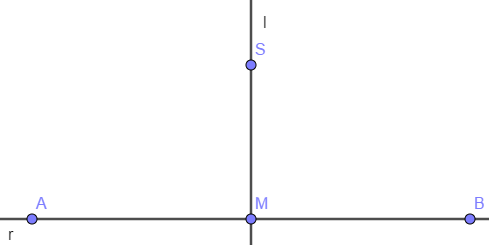
\includegraphics[width=7cm]{figuras/2-23.png}
	\vspace{-1em}
\end{figure}

\lema{2.21} Si $\sigma_r$ entonces, para todo $X$, $\m[X, \sigma_r(X)] \in r$.

\obs{2.24} Si $l \perp r$ y $g \in \iso(\P)$ entonces $g(l) \perp g(r)$.

\importante\tma{2.26} Si $l, r \subset \P$ cortan en $M$ y $\sigma_l, \sigma_r$ son dos reflexiones de $l$ y $r$, entonces se cumple que $l \perp_M r \iff r \perp_M l \iff \sigma_r(l) = l \iff \sigma_l(r) = r$.

\importante\tma{2.27 / 2.29} Para toda recta $r$ y todo punto $S \in \P - r$, existe una recta $l$ ortogonal a $r$, que pasa por $S$. Si $r$ es una recta, y $M \in r$, entonces existe $l$ tal que $l \perp_M r$.

\axioma{P7} Para toda recta $r$ y todo punto $P$ existe sólo una recta \textbf{paralela} a $r$ que pase por $P$.

\tma{2.31 / 2.33} Si $a \perp l$ y $b \perp l$ entonces $a \parallel b$. Sean $a \parallel b$. Entonces, para todo $A \in a$, la única recta $l \perp_A a$ también es ortogonal a $b$.

\tma{2.32} Las rectas parallelas forman una relación de equivalencia.
\begin{itemizex}
	\item Reflexividad: $a\parallel a$
	\item Simetría: $a \parallel b \rightarrow b \parallel a$
	\item Transitividad  $a \parallel b $ y  $b \parallel c \rightarrow a \parallel c$
\end{itemizex}

\ej{2.6} Sean $A,B \in r$, $A \neq B$. Para todo $t$, existe un único $P_t\in r$ que cumple $d(P_t,A) = \abs{t}$ y $d(P_t, B) = \abs{t-d(A,B)}$. En definitiva, la posición de $P_t$ está sólamente determinada por las distancias $d(A, P_t)$ y $d(P_t, B)$.
	 
	 
	 
	 
	 
	 
	 \end{multicols*}\pagebreak


	\begin{multicols*}{2}
	[\section{Isometrías del plano}]
	
\defi{3.1} Para una aplicación $\phi: \pazocal{M} \rightarrow \pazocal{M}$, $P\in \pazocal{M}$ es un \textbf{punto fijo} de $\phi$ si $\phi(P) = P$; y $\pazocal{D} \subset \pazocal{M}$ es un \textbf{subconjunto invariante} de $\phi$ si $\phi(\pazocal{D}) = \pazocal{M}$.

\lema{3.2} Si $g \in \iso(\P)$ y $A \neq B$ son dos puntos fijos de $g$, entonces todo $X \in r_{AB}$ es punto fijo de $g$.


\defi{3.3} Si $g, g' \in \iso(\P)$, $g$ y $g'$ son \textbf{conjugadas}
si existe una isometría $h$ tal que $gh = hg' \iff g = hg'h^{-1}$.

\tma{3.4} Un punto $P$ es fijo de $g$ sii $h^{-1}(P)$ es un punto fijo de $g'$.

\dem{Si $h^{-1}(P)$ es punto fijo de $g'$, entonces $g'(h^{-1}(P)) = h^{-1}(P)$. Por tanto, $g(P) = hg'h^{-1}(P) = hh^{-1}(P) = P$, luego $g(P) = P$.}

\ejem{3.5} Una reflexión sobre $r$ cumple que
\begin{itemizex}
	\item $\sigma_r\circ\sigma_r = \text{id}_{\P}$ y $\sigma_r(X) = X \iff X \in r$ (\axioma{P6})
	\item $\sigma_r(H^1) = H^2$ y viceversa.
	\item $X$ y $\sigma_r(X)$ se encuentran en una recta ortogonal a $r$.
\end{itemizex} 

\tma{3.6} Sea $g\in \iso(\P)$ y sea $r_{AB}$. Si $A, B$ son puntos fijos en $g$, entonces o bien $g = \sigma_r$ o bien $g = \text{id}_\P$. 

\tma{3.9} Llamamos $\rho$ una \textbf{rotación} a una isometría que tiene un punto fijo $C$. Para toda recta $a$ pasando por $C$ existen dos rectas $b, b'$ únicas tales que $\rho = \sigma_b\sigma_a = \sigma_a\sigma_{b'}$.

\begin{figure}[H]
	\centering
	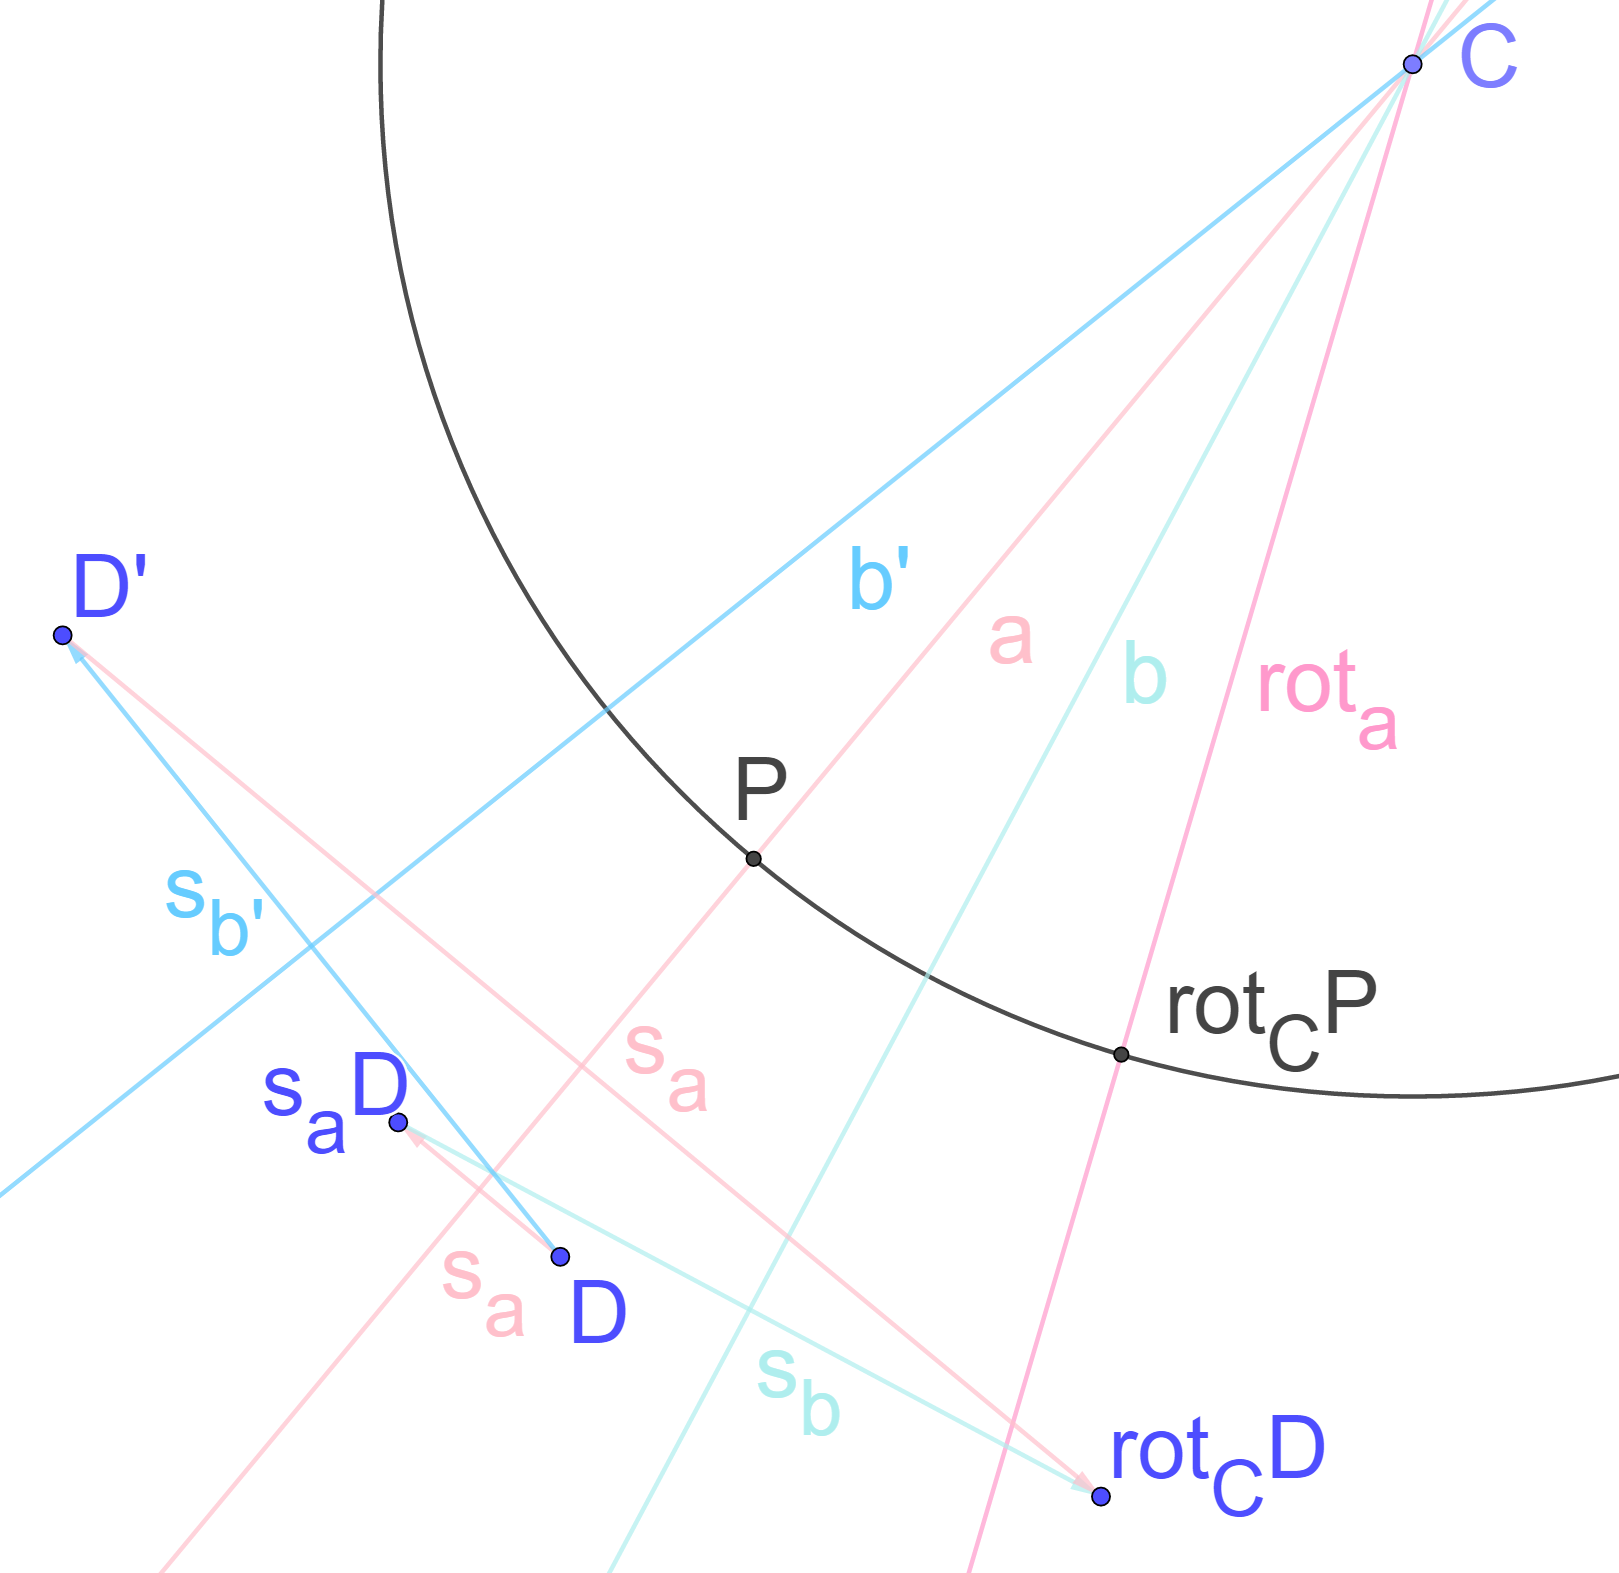
\includegraphics[width=7cm]{figuras/3-9.png}
	\vspace{-1em}
\end{figure}

\ej{3.1} Llamamos $\tau$ una \textbf{traslación} a una isometría que no tiene puntos fijos y deja una recta $c$ invariante, es decir, $\tau(c) = c$. entonces para toda recta $a\perp c$ existen dos rectas $b,b' \perp c$ que cumplen $\tau = \sigma_b\sigma_a = \sigma_a\sigma_{b'}$. Además, si $\tau(l) = l$, entonces $l \parallel c$.

\begin{figure}[H]
	\centering
	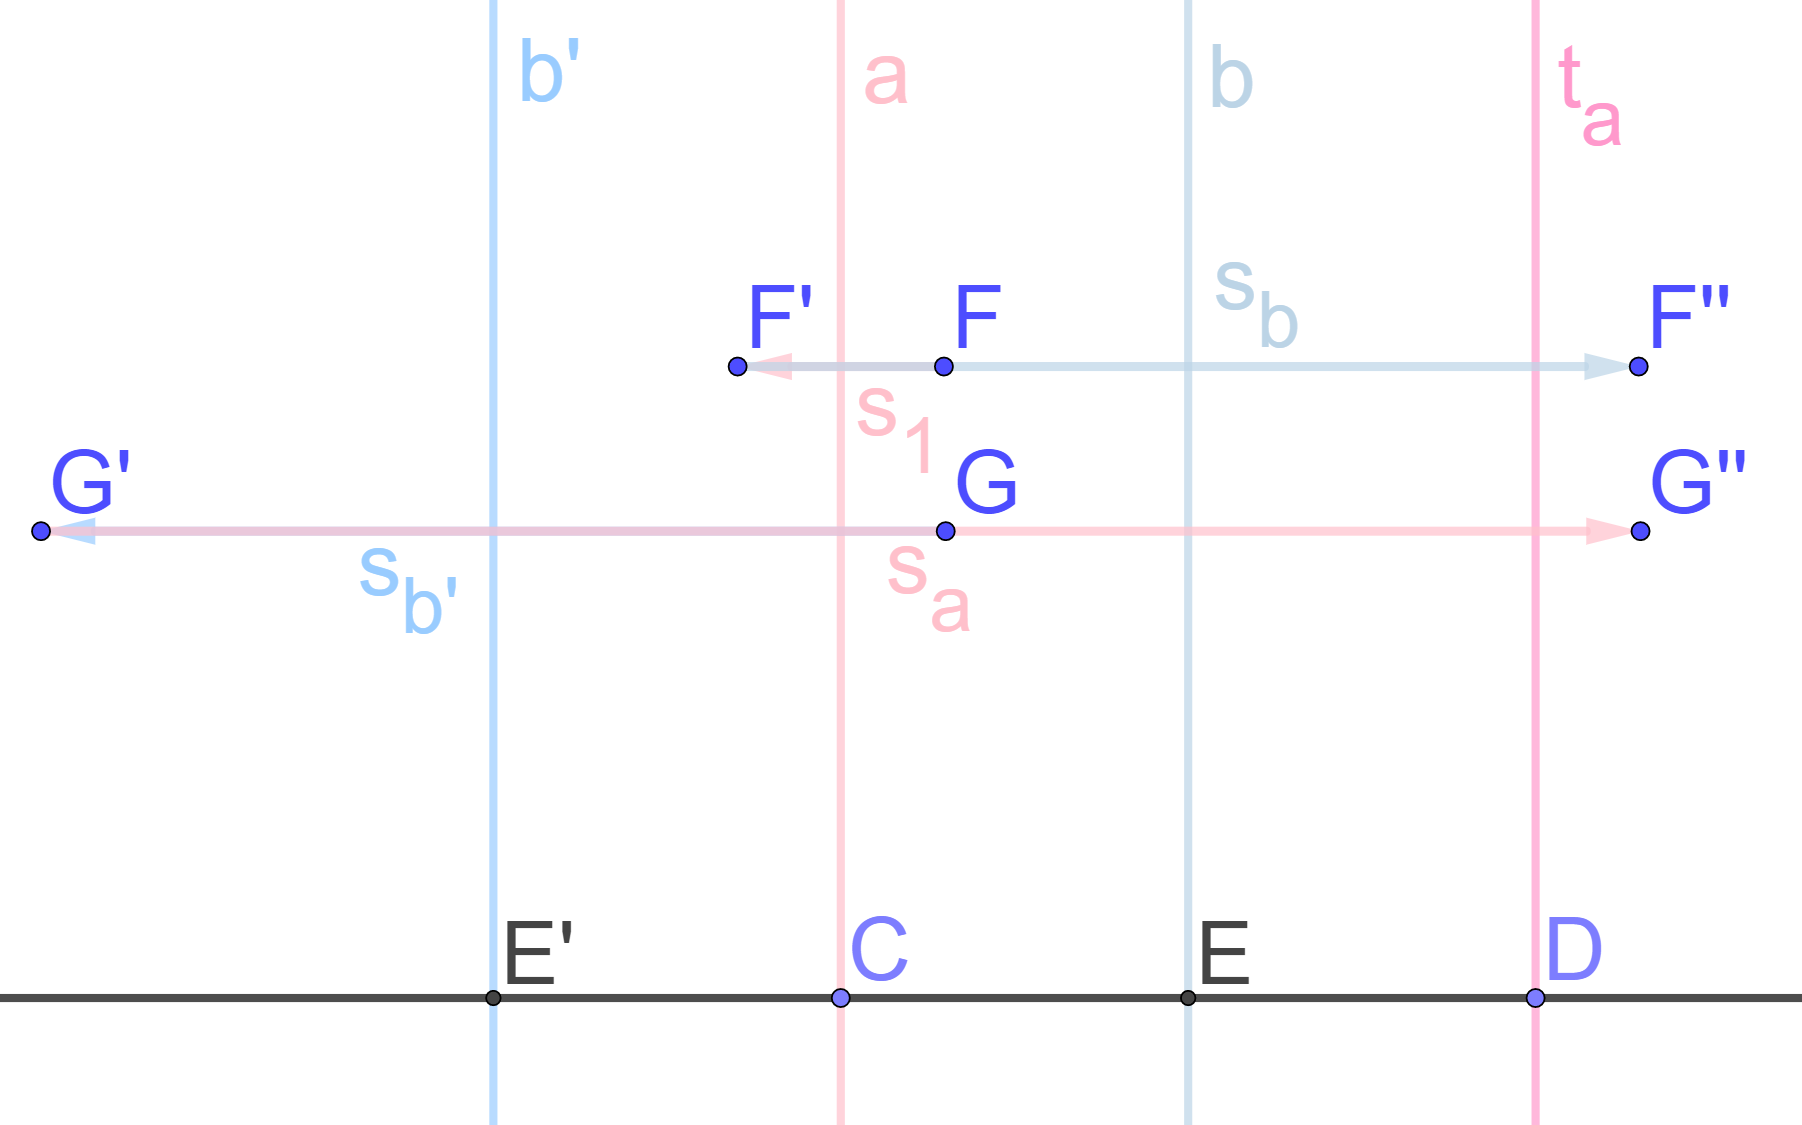
\includegraphics[width=7cm]{figuras/3-1.png}
	\vspace{-1em}
\end{figure}

\ej{3.2} Si $\pazocal{R}_P(\P) = \{g\in \iso(\P) \;|\; g \text{ es} $ 
	\linebreak
	rotación de centro $ P \} \cup \{ \text{id}_\P \}$ entonces
	\begin{itemizex}
		\item Si $a$ es una recta que pasa por $P$, entonces $g^{-1} = \sigma_a g \sigma_a$.
		\item $gh = hg$ para todo $g,h \in \pazocal{R}_P(\P)$.
		\item Para $X \in \P - \{P\}$ y $g(X) = h(X)$ entonces $g = h$.
	\end{itemizex}

\ej{3.3} Si $h$ es una isometría
 	\begin{itemizex}
 	\item Si $g \in \pazocal{R}_P(\P)$ entonces $hgh^{-1} \in \pazocal{R}_{h(P)}(\P)$
 	\item Si $r$ es una recta entonces $h\sigma_rh^{-1} = \sigma_{h(r)}$
	\end{itemizex}

\ej{3.3} Si $a, b$ son rectas en $\P$
	\begin{itemizex}
	 	\item $\sigma_a\sigma_b\sigma_a = \sigma_{a(b)}$
	 	\item $\sigma_a\sigma_b = \sigma_b\sigma_a \iff a \perp b$
	\end{itemizex}

\ejem{3.12} Sean $a,b$ tales que $a\perp_P b$. Entonces la rotación es de 180$^\circ$ y se
llama \textbf{reflexión central} si se denota como $\sigma_P$. Cumple las siguientes propiedades.
	\begin{itemizex}
		\item $\sigma_P\sigma_P= \text{id}_\P$
		\item Para todo $X$, $\sigma_P(X)$ es el único punto que cumple $P = \m[X, \sigma_P(X)]$.
		\item $\sigma_P$ es independiente de la elección de rectas $a\perp b$.
	\end{itemizex}

\tma{3.13} Las rectas $r$ y $\sigma_P(r)$ son paralelas.

\ejem{3.14} Una \textbf{reflexión con deslizamiento} $\phi$ es una composición de una reflexión $\sigma_c$ y una traslación $\tau$: $\phi = \tau\sigma_c$. $\phi$ deja invariante sólo la recta $c$, y no tiene ningún punto invariante.

\tma{3.15} Una isometría solo puede pertenecer a una de las de la tabla, y es una combinación de un número par o impar de reflexiones $\sigma$:

\begin{tabular}{l c c}
	& Con puntos fijos & Sin puntos fijos\\
	par & $\rho$ & $\tau$\\
	impar & $\sigma$ & $\phi$ \\
\end{tabular}


\tma{3.16} Si $g, g'$ son isometrías conjugadas, tienen la misma paridad.






	 
	 \end{multicols*}\pagebreak
	
	
	\begin{multicols*}{2}
	[\section{Ángulos}]
	\defi{4.1} Sean $r,l$ dos rectas con un punto $V$ en común. Sean $\overline{r}$ y $\overline{l}$ dos semirrectas determinadas por $V$ en $r$ y $l$. El par $\{\overline{l}, \overline{r} \}$ es un \textbf{ángulo}. $V$ es el vértice del ángulo y $\overline{l}$ y $\overline{r}$ son los lados del ángulo. El ángulo se designa por $\angle \{\overline{l}, \overline{r} \}$ o, si no hay lugar a confusión, $\angle V$. Así, por ejemplo, dado un triángulo $\triangle PQR$, $\angle P$ es el ángulo formado por $P$ con $[P,Q]$ y $[P,R]$.

\obs{4.4} Si $r = l$, y $\overline{r}_1$ y $\overline{r}_2$ son las semirrectas determinadas por $V$, entonces, en estas circunstancias, el ángulo $\angle\{ \overline{r}_1, \overline{r}_2 \}$ se denomina \textbf{ángulo llano} y $\angle\{ \overline{r}_1, \overline{r}_1 \}$ se denomina \textbf{ángulo nulo}.

\defi{4.5} Un ángulo $\angle \{\overline{l}, \overline{r} \}$ y un ángulo $\angle \{\overline{l}', \overline{r}' \}$ son \textbf{congruentes} si existe una isometría $g$ tal que $g(\{\overline{l}, \overline{r} \}) = \{\overline{l}', \overline{r}'\} $. Todos los ángulos que son congruentes forman una \textbf{clase de congruencia} de ángulos. Empleando la notación de vértices, la congruencia se denota como $\angle A = \angle B$.

\obs{4.6/4.8} Si  $\angle \{\overline{l}, \overline{r} \}$ tiene vértice $V$ y  $\angle \{\overline{l}', \overline{r}' \}$ tiene vértice $V'$, y $g$ es una isometría tal que $g(  \{\overline{l}, \overline{r} \}) =   \{\overline{l}', \overline{r}' \}$, entonces $g(V) = V'$. Asimismo, si existe una isometría $h$ que hace $h(V) = V'$, entonces  $h(  \{\overline{l}, \overline{r} \}) =   \{\overline{l}', \overline{r}' \}$.

\ejem{4.9} Consideramos las rectas $a \neq b$ que cortan en $V$, con sus respectivas semirrectas 
$\overline{a}_1, \overline{a}_2, \overline{b}_1, \overline{b}_2$. Consideramos $\angle \{\overline{a}_1, \overline{b}_1 \}$ y elegimos los puntos $A \in \overline{a}_1, B \in \overline{b}_1$ a igual distancia, $d(V,A) = d(V,B)$. Existe una recta $l \perp r_{AB}$ que pasa por $V$ (\tma{2.25/2.29}, que denominamos \textbf{bisectriz}. La bisectriz $l$ cumple que $\sigma_l(A) = B, \sigma_l(\overline{a}_1) = \overline{b}_1$ y viceversa. Además, si $\overline{l}$ es la semirrecta que corta a $[A,B]$, entonces $\angle \{\overline{a}_1, \overline{l} \} = \angle \{\overline{b}_1, \overline{l} \}$.

\tma{4.11} 

	 
	 \end{multicols*}\pagebreak
	
		
		\begin{multicols*}{2}
		[\section{Teorema de Tales}]
		\defi{5.0} Un \textbf{cuadrilátero} es una cuaterna ordenada de puntos [vértices] de $\P$, $(P, Q, R, S)$ formada por los segmentos $[P,Q], [Q,R], [R,S], [S,P]$ [lados] si dos cualesquiera segmentos son disjuntos o tienen un extremo en común. Dos vértices extremos del mismo lado son adyacentes y, si no, son opuestos.

\defi{5.1} Un cuadrilátero $\square PABC$ es un \textbf{paralelogramo} si $\m[P,B] = \m[A,C] = M$, donde los segmentos $[P,B]$ y $[A,C]$ son las diagonales, y $M$ es el centro.

\obs{5.2} Sea $\square PABC$ con centro $M$. Por las propiedades de las reflexiones centrales, se tiene que $\sigma_M(P) = B$ y $\sigma_M(A) = C$ [y viceversa]. Además, por tales propiedades, se tiene que $r_{PA} \parallel r_{BC}$ y $r_{PC} \parallel r_{AB}$; y $d(P,A) = d(B, C)$ y $d(P,C) = d(A,B)$. 

\obs{5.3} Si existen tres puntos $P,A,C$ no alineados, se puede construir un paralelogramo de varias maneras. Una forma es aplicar el axioma de las paralelas y proyectar $r_{PA}$ en $C$, y $r_{PC}$ en $A$. Otra forma es obtener $M  = \m[C,A]$, crear la recta $r_{PM}$ y proyectar el punto $B$ como el que $PM = d(P,M) = d(M,B) = MB$.

\obligatorio\tma{5.5 [Tales]} Sea $\triangle PAB$ y sean $A' \in [P,A]$, $B' \in  [P,B]$ dos puntos tales que $r_{AB} \parallel r_{A'B'}$. En estas condiciones se tiene que $\frac{PA'}{PA} = \frac{PB'}{PB}$.

\begin{figure}[H]
	\centering
	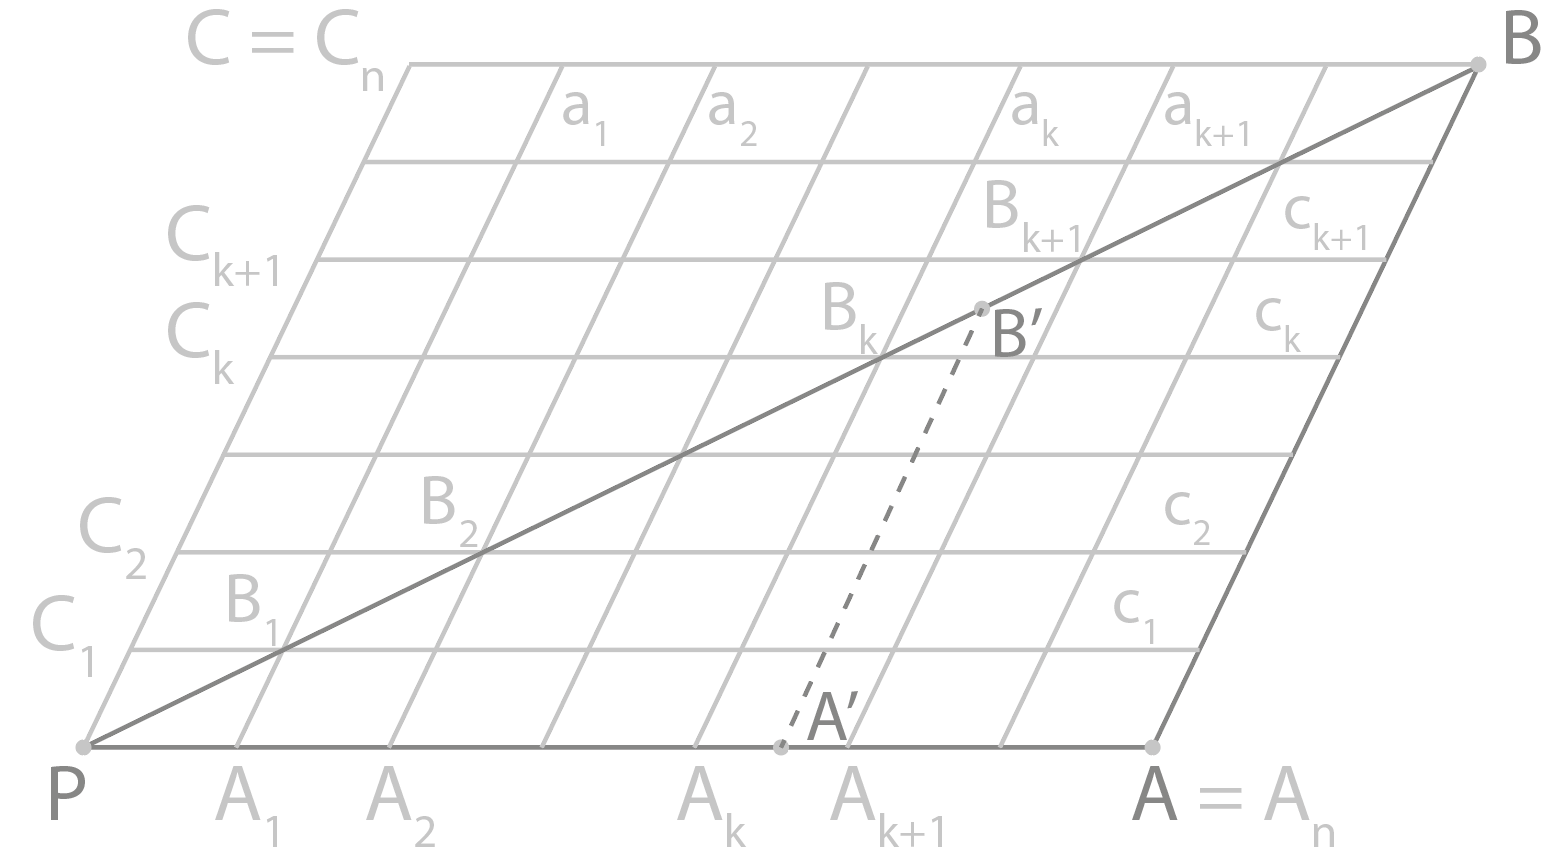
\includegraphics[width=8.2cm]{figuras/5-5.png}
	\vspace{-1em}
\end{figure}

\dem{Vamos a basar la demostración en la figura de arriba. 
Diseñamos el paralelogramo $\square PABC$ y dividimos el lado $[P,A]$ en $n$ segmentos con puntos de división $A_1, A_2, \cdots, A_n$, de modo que $d(A_i,A_{i+1}) = \frac{d(P,A)}{n}$. El mismo proceso se realiza con el lado $[P,C]$. Además, introducimos las rectas $a_k\parallel r_{PC}$ y $c_k\parallel r_{PA}$, de modo que el punto $P_{kl}$ es la intersección de $a_k$ con $c_l$. Vemos que $B_i = P_{ii}$. También observamos que existen los paralelogramos $\square A_kA_{k+1}P_{k+1,l}P_{k,l}$ y $\square C_lC_{l+1}P_{k,l+1}P_{k,l}$, de modo que $P_{kl}P_{k+1,l} = \frac{PA}{n}$ y $P_{kl}P_{k,l+1} = \frac{PC}{n}$.\linebreak
Ahora consideramos $B_k$. Sabemos que $\sigma_{B_k}(r) \parallel r$, $\sigma_{B_k}(c_k) = c_k$ y $\sigma_{B_k}(P_{k-1,k}) = P_{k+1,k}$. También, como $a_{k-1} \parallel a_{k+1}$, $\sigma_{B_k}(a_{k-1}) = a_{k+1}$, y por el mismo criterio, $\sigma_{B_k}(c_{k-1}) = c_{k+1}$. Con esto demostramos que $$\sigma_{B_k}(B_{k-1}) =\sigma_{B_k}(P_{k-1, k-1}) = P_{k+1, k+1}= B_{k+1}$$
Por tanto, los puntos $B_{k-1}, B_k, B_{k+1}$ están alineados y $B_{k-1}B_k = B_kB_{k+1}$. Por tanto, $B_kB_{k+1} = \frac{PB}{n}$.\linebreak
Es decir, hemos demostrado que
$$P_{kl}P_{k+1,l} = \frac{PA}{n} \quad  P_{kl}P_{k,l+1} = \frac{PC}{n} \quad P_{kl}P_{k+1,l+1} =  \frac{PB}{n}$$
Si reordenamos, tenemos que 
$$\frac{PA_k}{PA} = \frac{P_{0,0}P_{k,0}}{PA} = \frac{k}{n} = \frac{P_{0,0}P_{k,k}}{PB} =  \frac{PB_k}{PB}$$
Y con esto demostramos el teorema para los puntos $k$. Si tenemos $A'$ y $B'$ en la figura tales que $A' \in [A_k, A_{k+1}]$, de modo que $a' = r_{A'B'}$ está entre $a_k$ y $a_{k+1}$, y es paralelo a estas, haciendo que $B' \in [B_k, B_{k+1}]$. Por ser $A' \in [A_k, A_{k+1}]$ entonces $\frac{PA_k}{PA} \le \frac{PA'}{PA} \le \frac{PA_k}{PA}+\frac{1}{n}$ y, como $\frac{PA_k}{PA} = \frac{PB_k}{PB}$, entonces $\frac{PB_k}{PB} \le \frac{PA'}{PA} \le \frac{PB_k}{PB}+\frac{1}{n}$. Dado que $B'\in [B_k,B_{k+1}]$ entonces
$$\textcolor{SkyBlue}{\frac{PB'}{PB}-\frac{1}{n}} \le \frac{PB_k}{PB} \le \textcolor{SkyBlue}{\frac{PA'}{PA}} \le \frac{PB_k}{PB}+\frac{1}{n} \le \textcolor{SkyBlue}{\frac{PB'}{PB}+\frac{1}{n}}$$ 
Si nos fijamos en los elementos de azul, vemos que $n$ puede hacerse tan pequeño como queramos, de modo que, en el límite
$$\frac{PB'}{PB} \le \frac{PA'}{PA} \le \frac{PB'}{PB} \iff \frac{PB'}{PB} = \frac{PA'}{PA}$$ }

\cor{5.6} En base al teorema de Tales, se tiene que 
$$\frac{PA'}{PA} = \frac{PB'}{PB} = \frac{A'B'}{AB}$$

\defi{5.7} Dado un triángulo rectángulo $\triangle PAB$ con $\angle A$ recto, entonces la \textbf{hipotenusa} es el lado opuesto a $\angle A$, $[P,B]$. Los lados adyacentes, $[P,A],[B,A]$, son los \textbf{catetos}.
\begin{figure}[H]
	\centering
	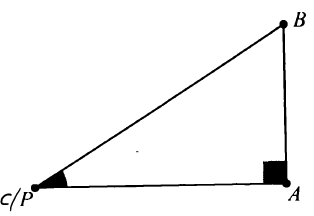
\includegraphics[width=3.5cm]{figuras/5-7.png}
	\vspace{-1em}
\end{figure}
\defi{5.8} Sea el triángulo rectángulo $\triangle PAB$ con $\angle A$ recto, entonces se definen las relaciones 
\begin{itemize}
	\item seno: $\text{sen}\angle P = \frac{BA}{PB}$
	\item coseno: $\text{cos}\angle P = \frac{PA}{PB}$
	\item tangente: $\text{tan}\angle P = \frac{BA}{PA}$
	\item cotangente: $\text{cot}\angle P = \frac{PA}{BA}$
\end{itemize}
\tma{5.10} Las razones trigonométricas para $\angle P$ no dependen del triángulo $\triangle PAB$, sólo de la clase de congruencia de $\angle P$.

\tma{5.12} Dado un triángulo rectángulo $\triangle ABC$ con $\angle A$ recto, la medida de los catetos, $AB,AC$, es menor que la de la hipotenusa $BC$.
\begin{figure}[H]
	\centering
	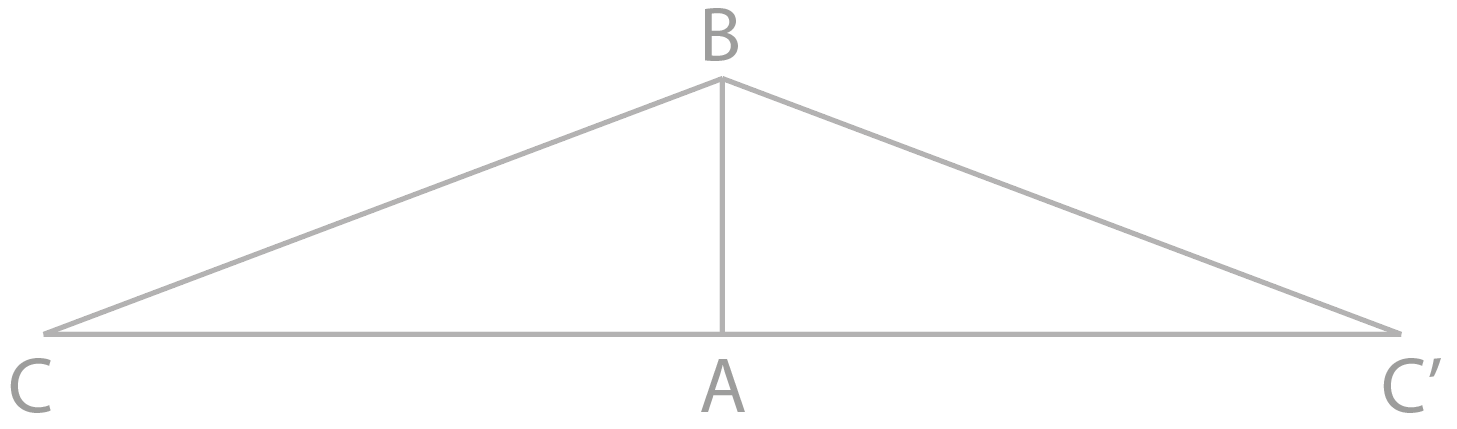
\includegraphics[width=6.5cm]{figuras/5-12.png}
	\vspace{-1em}
\end{figure}
\dem{Con la construcción anterior, vemos que los puntos $B, C, C'$ no están alineados, pues $C \in r_{AC}$ y $r_{AB}\perp r_{AC}$. Por la desigualdad triangular tenemos que $2AC = CC' < BC+BC' = 2BC$.}

\defi{5.13} La \textbf{medida de un ángulo} agudo $\angle P$ es el número real:
$$\measuredangle P = \arccos(\cos \angle P)$$
\tma{5.14 / 5.19} Si $\angle P = \angle Q$ entonces $\measuredangle P = \measuredangle Q$, sean $\angle P $ y $\angle Q$ agudos y obtusos.

\defi{5.15} Dado un ángulo $\angle{\overline{a}, \overline{b}_1} = \angle V$, un \textbf{ángulo suplementario} $\overline{\angle V} = \angle{\overline{a}, \overline{b}_2}$ es aquel donde $\overline{b}_1$ y $\overline{b}_2$ son las dos semirrectas de $b$ en $V$, y $\angle V$ y $\overline{\angle V}$ comparten $\overline{a}$. La suma de $\angle V$ y $\overline{\angle V}$ es un ángulo llano.

\tma{5.17} Si dos ángulos son congruentes, sus suplementarios lo son.

\defi{5.18} Para un ángulo obtuso $\angle P$ se tiene $\sen \angle P = \sen \overline{\angle P}$ y $\cos \angle P = -\cos \overline{\angle P}$

\end{multicols*}\pagebreak
	
	
	
	 \noindent\rule{\linewidth}{0.4pt}
	 \doclicenseThis
	 
	 
	 
	 
	 
	 
	 
	 
	  	
 	
 	
 	
 	
 	
\end{document}